\chapter{Methode}
\section{Conceptueel ontwerp}
In dit hoofdstuk wordt het ontwerp en de realisatie van de ontworpen pipet besproken. Hierbij worden de verschillende onderdelen behandeld, als ook de gemaakte keuzes. 
\subsection{Literatuurstudie}
De Literatuurstudie bestond voor een groot deel uit het bestuderen van beschikbare patenten. Patenten zoals\ \cite{RN16} en\ \cite{RN17} beschrijven analoge pipetten. Deze patenten waren belangrijk om de basiswerking van moderne pipetten te begrijpen.
Verder werden de patenten \ \cite{RN35} en\ \cite{RN36} bestudeerd. Deze patenten beschrijven de werking van een motorisch aangedreven, elektronische, pipet.
\section{Hardware ontwerp}
\begin{center}
    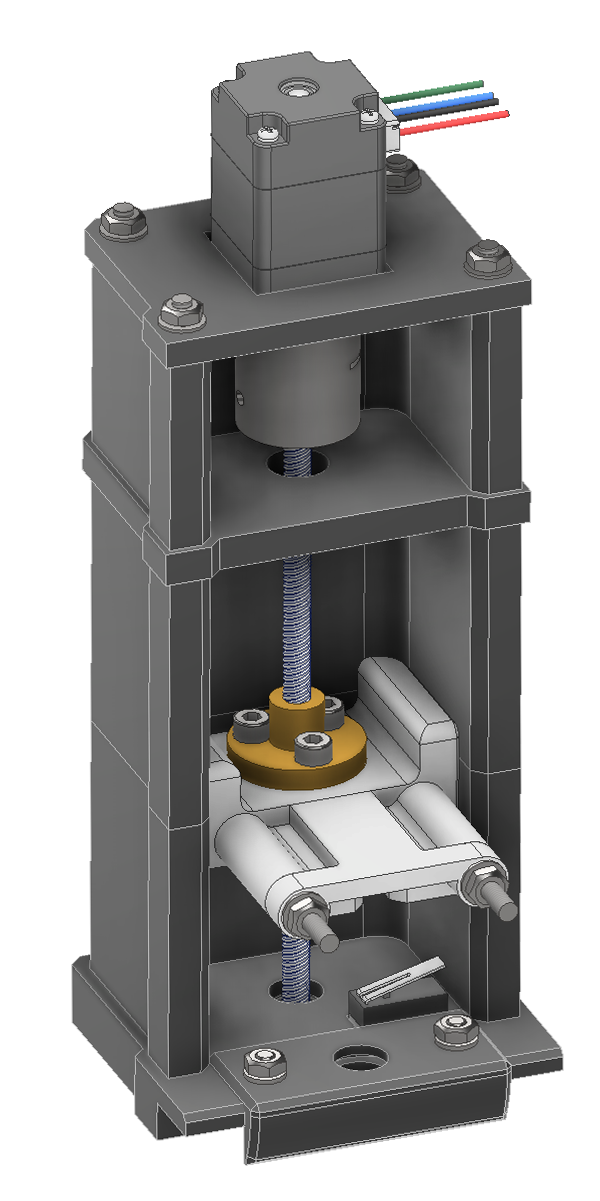
\includegraphics[height=9cm]{figures/FullModel.png}
\end{center}
\section{Elektronica ontwerp}
\section{Software ontwerp}

